\documentclass[11pt, oneside]{article}
\usepackage[margin=1in,letterpaper]{geometry}
\usepackage{times}
\usepackage{graphicx}
\usepackage{amssymb,amsmath}
\usepackage{array}
\usepackage{longtable}
\usepackage{color}
\usepackage[T1]{fontenc}
\usepackage{sectsty}
\usepackage{tikz}
\usepackage{pgfplots}
\pgfplotsset{compat=1.17}
\sectionfont{\fontsize{12}{12}\selectfont}
\subsectionfont{\fontsize{11}{11}\selectfont}
\subsubsectionfont{\normalsize\itshape\mdseries}

\renewcommand\labelitemi{{\boldmath$\cdot$}}

%%%%%%%%%%%%%%%%%%%%%%%%%%%%%%%%%%%%%

\title{12.421/12.621 Lecture 1: Material Properties}
\author{Brent Minchew}
\date{}

\begin{document}
\maketitle

\noindent\textbf{Topics covered}
\begin{itemize}
	\item Constitutive parameters
	\item Permittivity and material polarization
	\item Simple models for the permittivity of water and water ice
\end{itemize}

%%%%%%%%%%%%%%%%%%%%%%%%%%%%%%%%%%%%%
\section{Inferences from remote sensing data}

\begin{itemize}
	\item It is often the case that we want to infer physical properties of observed areas on Earth or other bodies from remote sensing (RS) data.
	\item In this course (and in general), we have defined RS methods as those that utilize electromagnetic (EM) radiation.
	\item The EM radiation of interest in this course is either emitted from, or has interacted with, the medium of interest.
	\item Our goal throughout most of this course, then, is to develop a foundational understanding of and intuition for the interaction of EM radiation with matter.
	\item This will be done through several broad topics, starting with, in order:
	\begin{enumerate}
		\item Constitutive parameters
		\item Classical EM principles (Maxwell's equations)
		\item Wave propagation
	\end{enumerate}
	\item Today, we cover constitutive parameters.
\end{itemize}

%%%%%%%%%%%%%%%%%%%%%%%%%%%%%%%%%%%%%
\section{Constitutive parameters}

The EM characteristics of any material can be described by four constitutive parameters:
\begin{enumerate}
	\item $\bigstar$ $\varepsilon'\varepsilon_0$ is the electrical \emph{permittivity}
	\begin{itemize}
		\item measure of a material's ability to store an electric charge
		\item units: F/m, where F = Farad = J/V$^2$ is a unit of capacitance
		\item written above as the product of two parameters:
		\begin{itemize}
			\item $\varepsilon_0 = 8.85\times10^{-12}$ F/m is the permittivity of free space
			\item $\varepsilon' = \varepsilon_\mathrm{material}/\varepsilon_0$ is the (dimensionless) relative permittivity (relative to free space)
			\item it is almost always the case that $\varepsilon' \ge 1$ (exceptions discussed later)
			\item $\varepsilon'$ is of \emph{fundamental importance in RS} and is something we delve into more in this lecture
		\end{itemize}
	\end{itemize}
	% NOTE: handwritten uses rho_v for charge density; written q_v so that rho is reserved for reflection
	% coefficients (Lecture 4 onward, following Ulaby & Long). Instructor decision, 2026-09-29.
	\item $q_v$ is the \emph{charge density}
	\begin{itemize}
		\item units: C/m$^3$, where C = Coulomb = A$\cdot$s
		\item $q_v = 0$ for RS applications, so it is not considered further in this course
	\end{itemize}
	\item $\mu$ is the magnetic \emph{permeability}
	\begin{itemize}
		\item measure of a material's ability to support the development of a magnetic field
		\item units: H/m, where H = Henry = J/A$^2$ is a unit of inductance
		\item $\mu_0 = 4\pi\times10^{-7}$ H/m is the permeability of free space
		\item $\mu = \mu_0$ in virtually all RS applications, so it will not be considered further in this course
		\item $c = 1/\sqrt{\mu_0\varepsilon_0}$ is the speed of light in a vacuum
	\end{itemize}
	\item $\bigstar$ $\sigma$ is the \emph{conductivity}
	\begin{itemize}
		\item measure of a material's ability to allow current to flow through it
		\item accounts for EM wave attenuation in materials, and is therefore of \emph{fundamental importance in RS}
		\item units: S/m, where S = Siemens = $\Omega^{-1}$ = A/V
		\item general categories and examples:
		\begin{itemize}
			\item $\sigma = 0$: ``lossless'' (e.g., vacuum)
			\item $\sigma \approx 0$: ``low-loss'' (e.g., air)
			\item $\sigma > 0$: ``lossy'' (e.g., seawater)
			\item $\sigma \gg 1$: ``conductor'' (e.g., copper, gold)
			\item $\sigma \to \infty$: ``perfect conductor''
		\end{itemize}
	\end{itemize}
\end{enumerate}

\subsection{The complex dielectric constant}

For RS applications, $\mu \approx \mu_0$ and $q_v = 0$, so we are mainly concerned with $\varepsilon'\varepsilon_0$ and $\sigma$. We combine these into a single, complex-valued parameter, the (dimensionless, complex) \emph{dielectric constant}
\begin{equation}
	\label{e:dielectric}
	\varepsilon = \varepsilon' - j\varepsilon'', \qquad \text{where} \qquad \varepsilon'' = \frac{\sigma}{\omega\varepsilon_0} \qquad (j^2 = -1)
\end{equation}
and $\omega$ is the (angular) frequency of the EM wave. The derivation of $\varepsilon$ will be done later in the course.
% NOTE: added scope (instructor decision, 2026-09-29). sigma/(omega eps_0) is the conduction contribution to eps''; polarization
% (relaxation) losses also contribute, e.g., pure water (sigma ~ 0) has a Debye eps'' ~ 10.5 at 2.45 GHz and 20 C (Section 5).
Here $\sigma/(\omega\varepsilon_0)$ is the contribution of conduction to $\varepsilon''$. Polarization (relaxation) mechanisms also add to $\varepsilon''$, as we will see in Section~\ref{s:water}.

Comments on $\varepsilon$:
\begin{itemize}
	\item $\varepsilon'$ has already been discussed (relative permittivity).
	\item $\varepsilon''$ is the \emph{loss factor}, which represents attenuation of the EM wave.
	\begin{itemize}
		\item In general, RS applications involve narrow ranges of $\omega$ (and $\varepsilon_0$ is a universal constant).
		% NOTE: handwritten reads "attenuation is governed primarily by sigma" and "attenuation occurs through heating"; scoped to
		% conduction losses and reworded (absorbed energy becomes heat, not the reverse). Instructor decision, 2026-09-29.
		\item Therefore, conduction losses are governed by the conductivity $\sigma$.
		\item The absorbed energy is converted to heat; this is how microwave ovens work (through both the dipolar-relaxation and the ionic-conduction losses of water).
	\end{itemize}
	\item Taking a broader view of RS, where the range of $\omega$ is large, we have $\varepsilon'(\omega)$ and $\sigma(\omega)$.
	\item Several mechanisms by which $\varepsilon'$ and $\sigma$ vary with $\omega$ will be covered throughout the course, but these can be classified mainly as stretching and rotating of atoms and molecules.
	\begin{itemize}
		\item Going through these will give some physical insight into the surprisingly complicated transparency of the atmosphere at different EM frequencies.
	\end{itemize}
	\item For now, let's keep things simple and build some intuition.
\end{itemize}

%%%%%%%%%%%%%%%%%%%%%%%%%%%%%%%%%%%%%
\section{Electric fields in matter}

\subsection{Conduction}

Conduction is something that everyone should have some broad understanding of: it is simply the ability of a material to allow the flow of electric current. Electric current is simply the movement of charged particles: electrons and/or ions.
\begin{itemize}
	\item So, conduction is a description of the ability of electrons and/or ions to move in a material.
	\item Metals, of course, are examples of excellent conductors.
	\item In RS applications, seawater is the ubiquitous example of a highly conductive natural material.
	\begin{itemize}
		% NOTE: handwritten reads "loss factor Imag(eps)"; written as eps'' since Im(eps) = -eps'' under eps = eps' - j eps''.
		\item We might therefore expect the loss factor $\varepsilon''$ to be high in seawater (more on this in a bit).
	\end{itemize}
\end{itemize}

\subsection{Permittivity}

In dielectric materials (i.e., insulators), charges are attached to specific atoms or molecules and are not free to ``roam.''
\begin{itemize}
	\item Charges can only move \emph{within} the atom or molecule.
	\item The cumulative effect of these small motions accounts for the characteristic behavior of dielectrics: permittivity.
	\item Remember that these motions are simply rotation and extension.
\end{itemize}

\subsubsection{Parallel-plate capacitor}

Let's dig into this a bit more by considering the simplest case of a parallel-plate capacitor.
\begin{itemize}
	\item Suppose we have two conductive plates of area $A$ separated by a distance $h$ and a perfect vacuum.
	\item Let's give the top plate a positive charge $+Q$ and the bottom plate a negative charge $-Q$ (Figure~\ref{f:capacitor}).
	\item The positively charged plate produces an electric field $E_+ = Q/(2A\varepsilon_0)$ that points away from the upper plate.
	\item The negatively charged plate does the opposite.
	\item Thus, there is a net field $E = Q/(A\varepsilon_0)$ between the two plates ($E=0$ outside the plates).
	\item The potential between the plates is then $V = Qh/(A\varepsilon_0)$.
	\item The capacitance is simply
	\begin{equation}
		\label{e:capacitance}
		C = \frac{Q}{V} = \frac{A\varepsilon_0}{h}.
	\end{equation}
\end{itemize}

\begin{figure}[h]
	\centering
	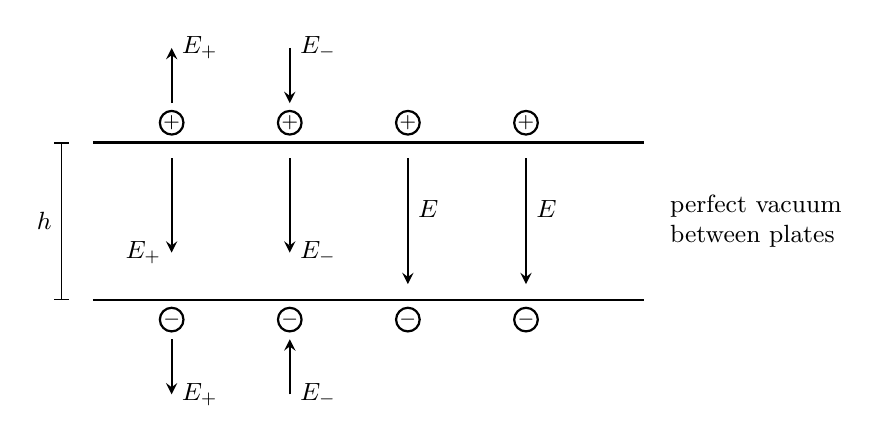
\begin{tikzpicture}[>=stealth, thick, font=\small]
		% plates
		\draw (0,2) -- (7,2);
		\draw (0,0) -- (7,0);
		% charges
		\foreach \x in {1,2.5,4,5.5} {
			\draw (\x,2.25) circle (0.15) node {\scriptsize $+$};
			\draw (\x,-0.25) circle (0.15) node {\scriptsize $-$};
		}
		% fields from + plate
		\draw[->] (1,2.5) -- (1,3.2) node[right] {$E_+$};
		\draw[->] (1,1.8) -- (1,0.6) node[left] {$E_+$};
		\draw[->] (1,-0.5) -- (1,-1.2) node[right] {$E_+$};
		% fields from - plate
		\draw[->] (2.5,3.2) -- (2.5,2.5) node[pos=0,right] {$E_-$};
		\draw[->] (2.5,1.8) -- (2.5,0.6) node[right] {$E_-$};
		\draw[->] (2.5,-1.2) -- (2.5,-0.5) node[pos=0,right] {$E_-$};
		% net field
		\draw[->] (4,1.8) -- (4,0.2) node[pos=0.4,right] {$E$};
		\draw[->] (5.5,1.8) -- (5.5,0.2) node[pos=0.4,right] {$E$};
		% separation
		\draw[|-|, thin] (-0.4,2) -- (-0.4,0) node[midway,left] {$h$};
		\node[align=left, anchor=west] at (7.2,1) {perfect vacuum\\between plates};
	\end{tikzpicture}
	\caption{Side view of a parallel-plate capacitor with a perfect vacuum between the plates. The fields from the two plates add between the plates and cancel outside.}
	\label{f:capacitor}
\end{figure}

We can see from Eq.~\eqref{e:capacitance} that $C \propto \varepsilon_0$. Recall that we placed a perfect vacuum between our plates, so we might suppose that the general relation is $C \propto \varepsilon'\varepsilon_0$.
\begin{itemize}
	\item Recalling that $\varepsilon' \ge 1$, we see that increasing permittivity increases capacitance.
	\begin{itemize}
		\item Countless observations back this up.
		\item You may have personal experience with this, as commercial capacitors always come with some insulator between the conductors.
	\end{itemize}
\end{itemize}

\subsubsection{Parallel-plate capacitor with a dielectric}

To see why this is, let's fill our parallel-plate capacitor with a dielectric.
\begin{itemize}
	\item Let's choose a simple, ubiquitous dipole molecule: H$_2$O.
	% NOTE: handwritten reads "Because H2O is a symmetric w/ 2 H atoms oriented at an angle of 104.5 deg"; reworded as asymmetric/bent.
	\item Because H$_2$O is asymmetric, with its two H atoms oriented at an angle of 104.5$^\circ$ from one another, it behaves as an electric dipole with its own field $E_{\mathrm{H_2O}}$ (Figure~\ref{f:water}a).
	\item In the absence of an external electric field, H$_2$O molecules are randomly oriented.
	\item If we place these between the plates of our capacitor, they orient themselves with the electric field of the capacitor (Figure~\ref{f:water}b).
	\item $E_{\mathrm{H_2O}}$ opposes $E$, which reduces the \emph{net} field.
	\begin{itemize}
		\item Electrical energy is stored in the ``polarization'' (orientation of molecules) of the dielectric.
	\end{itemize}
\end{itemize}
This is \emph{permittivity} in a nutshell.

\begin{figure}[h]
	\centering
	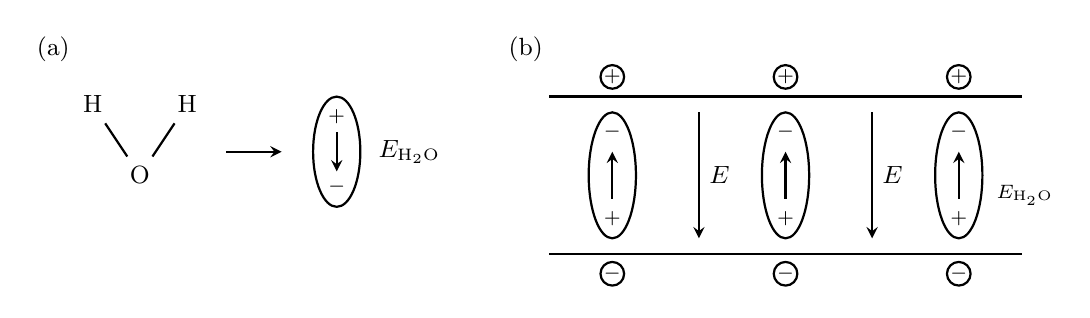
\begin{tikzpicture}[>=stealth, thick, font=\small]
		% (a) water molecule -> dipole
		\begin{scope}
			\node at (-0.3,2.6) {(a)};
			\node (O) at (0.8,1.0) {O};
			\node (H1) at (0.2,1.9) {H};
			\node (H2) at (1.4,1.9) {H};
			\draw (O) -- (H1);
			\draw (O) -- (H2);
			\draw[->] (1.9,1.3) -- (2.6,1.3);
			\draw (3.3,1.3) ellipse (0.3 and 0.7);
			\node at (3.3,1.75) {\scriptsize $+$};
			\node at (3.3,0.85) {\scriptsize $-$};
			\draw[->] (3.3,1.55) -- (3.3,1.05);
			\node[anchor=west] at (3.7,1.3) {$E_{\mathrm{H_2O}}$};
		\end{scope}
		% (b) capacitor with aligned dipoles
		\begin{scope}[xshift=6cm]
			\node at (-0.3,2.6) {(b)};
			\draw (0,2) -- (6,2);
			\draw (0,0) -- (6,0);
			\foreach \x in {0.8,3.0,5.2} {
				\draw (\x,2.25) circle (0.15) node {\scriptsize $+$};
				\draw (\x,-0.25) circle (0.15) node {\scriptsize $-$};
				\draw (\x,1) ellipse (0.3 and 0.8);
				\node at (\x,1.55) {\scriptsize $-$};
				\node at (\x,0.45) {\scriptsize $+$};
				\draw[->] (\x,0.7) -- (\x,1.3);
			}
			\draw[->] (1.9,1.8) -- (1.9,0.2) node[pos=0.5,right] {$E$};
			\draw[->] (4.1,1.8) -- (4.1,0.2) node[pos=0.5,right] {$E$};
			\node[anchor=west] at (5.55,0.75) {\scriptsize $E_{\mathrm{H_2O}}$};
		\end{scope}
	\end{tikzpicture}
	\caption{(a) The H$_2$O molecule acts as an electric dipole with field $E_{\mathrm{H_2O}}$. (b) Between the plates of a capacitor, the dipoles align with the capacitor's field $E$, and $E_{\mathrm{H_2O}}$ opposes $E$.}
	\label{f:water}
\end{figure}

\subsubsection{What the simple example leaves out}

This is a highly simplified example meant to show the fundamental concepts. There are several important elements missing:
\begin{enumerate}
	\item \textbf{Heat.} Vibrations associated with heat make perfect alignment of atoms or molecules impossible. Permittivity will therefore, in general, depend on temperature.
	\item \textbf{Impurities.} Rarely in RS will you look at pure materials. Impurities or other inclusions have major influences on the effective permittivity. For example:
	\begin{itemize}
		\item electrolytic solutions like salt water, where ionic salts increase conductivity by providing charges (ions) that can move large distances, producing an electric current;
		\item heterogeneous mixtures like wet or dry soil and snow.
	\end{itemize}
	\item \textbf{Dynamics.} The previous example was static, but in RS we care about the response of materials to \emph{oscillating} electric fields.
	\begin{itemize}
		\item Because the field is oscillating, we need to consider the response time of atoms and molecules to the electric field. We will call this response time the ``relaxation time.''
		\item Different mechanisms that influence permittivity have different relaxation times, so the dominant mechanism is governed by $\omega$:
		\begin{itemize}
			\item \emph{electronic or atomic polarization}: displacement of electron orbits relative to the nucleus $\rightarrow$ highest frequencies
			\item \emph{ionic polarization}: displacement of ion bonds in crystals $\rightarrow$ high frequencies
			\item \emph{dipolar polarization} (just discussed in the capacitor example): orientation of molecular dipoles $\rightarrow$ low frequencies
			\item \emph{interfacial (Maxwell--Wagner) polarization}: build-up of charge at boundaries between grains or materials with different electrical properties $\rightarrow$ lowest frequencies
		\end{itemize}
	\end{itemize}
\end{enumerate}

\subsection{A simple model for the response of materials to oscillating fields}

Here we approximate the response of materials to oscillating fields using classical mechanics.
\begin{itemize}
	% NOTE: handwritten uses x for the displacement and gamma for the damping coefficient; written as xi and nu to keep
	% x for Cartesian coordinates and gamma for the propagation constant (Lecture 2; master table D9, D13).
	\item To build some intuition, let us consider that electrons in an atom, molecules in a crystal, and dipoles in a mixture are bound by a force that can be treated (for small displacements) as a spring with constant $K_\mathrm{spring}$:
	\begin{equation}
		F_\mathrm{bond} = -K_\mathrm{spring}\,\xi = -m\omega_0^2 \xi,
	\end{equation}
	where $m$ is the mass of our particle and $\omega_0$ is the natural frequency.
	\item Let us also suppose there will be some damping mechanism (e.g., a friction-like force as in our capacitor example above, radiation in the case of atomic excitations, etc.; all will be covered in due course during the term). Damping must act opposite the velocity of the particle, and we \emph{assume} (to be justified later in the course) that it is proportional to velocity:
	\begin{equation}
		F_\mathrm{damping} = -m\nu\frac{d\xi}{dt}.
	\end{equation}
	% NOTE: handwritten writes the driving force as q E e^{j omega t}; written with Re[.] so the physical field is real, as in the
	% phasor box of Lecture 2 (instructor decision, 2026-09-29; master table D2).
	\item The driving force is related to our oscillating electric field:
	\begin{equation}
		F_\mathrm{driving} = qE(t) = q\,\mathrm{Re}\left[\tilde{E}e^{j\omega t}\right],
	\end{equation}
	where $q$ is the charge and $\tilde{E}$ is the complex amplitude (phasor) of the oscillating field.
	\item Newton's second law gives
	\begin{equation}
		m\frac{d^2\xi}{dt^2} = F_\mathrm{bond} + F_\mathrm{damping} + F_\mathrm{driving}
		\quad\Rightarrow\quad
		\frac{q}{m}E(t) = \frac{d^2\xi}{dt^2} + \nu\frac{d\xi}{dt} + \omega_0^2 \xi,
	\end{equation}
	which is a damped harmonic oscillator.
	\item This equation has a solution $\xi(t) = \mathrm{Re}[\tilde{\xi}e^{j\omega t}]$, where $\tilde{\xi}$ is the complex amplitude (\emph{phasor}) of the displacement (phasors are explained in a box in Lecture 2, Section 3.2). Because the equation is linear, each time derivative becomes a factor $j\omega$ acting on the phasors, so
	\begin{equation}
		\frac{q}{m}\tilde{E} = -\omega^2 \tilde{\xi} + j\omega\nu \tilde{\xi} + \omega_0^2 \tilde{\xi}.
	\end{equation}
	Solving for $\tilde{\xi}$ yields
	\begin{equation}
		\label{e:displacement}
		\tilde{\xi} = \frac{(q/m)\tilde{E}}{\omega_0^2 - \omega^2 + j\omega\nu}.
	\end{equation}
	% NOTE: the explanations of the dipole moment, the polarization, and Eq. (e:PE), and the display of Eq. (e:PE), were added
	% at the instructor's request (2026-10-01). The handwriting defines p~ = q xi~ and P~ = N p~ = N q xi~ and states
	% "In all cases encountered in RS, we have P~ = eps_0 (eps - 1) E~" inline.
	\item Each displaced charge $q$, together with the equal and opposite charge it is bound to (the nucleus for an electron cloud, a neighboring ion in a crystal, the other end of a polar molecule), forms an electric dipole. A dipole is characterized by its dipole moment: the charge times the separation of the two charges, pointing from the negative to the positive charge. Displacing the charge by $\xi$ from its equilibrium position therefore creates (or, for a permanent dipole such as H$_2$O, changes) a dipole moment $p = q\xi$ (units C$\cdot$m). Let us define the (complex amplitude of the) dipole moment $\tilde{p} = q\tilde{\xi}$.
	\item A single dipole is far too small to matter on its own; what the EM wave ``sees'' is the combined effect of all the dipoles in a volume. If there are $N$ dipoles per unit volume, all driven by the same field, their moments add, and the dipole moment per unit volume, or polarization per unit volume, is
	\begin{equation}
		\label{e:P}
		\tilde{P} = N\tilde{p} = Nq\tilde{\xi},
	\end{equation}
	where $N$ is the number of dipoles per unit volume.
	\begin{itemize}
		% NOTE (added): bound surface charge density = P . n-hat; with P along E (from the + plate toward the - plate), the face
		% next to the + plate carries -P and the face next to the - plate carries +P.
		\item $P$ has units of C/m$^2$, those of a surface charge density, and that is a useful way to picture it. In our capacitor example (Figure~\ref{f:water}b), the aligned dipoles leave a layer of bound charge on each face of the dielectric, $-P$ against the positive plate and $+P$ against the negative plate. This bound charge partly cancels the free charge $\pm Q/A$ on the plates, which is why the net field is reduced.
	\end{itemize}
	\item In all cases encountered in RS, the polarization is proportional to the field, and we write
	\begin{equation}
		\label{e:PE}
		\tilde{P} = \varepsilon_0(\varepsilon - 1)\tilde{E}.
	\end{equation}
	Why should $\tilde{P}$ be related to $\tilde{E}$ in this way?
	\begin{itemize}
		\item Proportionality: Eq.~\eqref{e:displacement} shows that $\tilde{\xi} \propto \tilde{E}$, so $\tilde{p}$ and $\tilde{P}$ are also proportional to $\tilde{E}$. The response is linear because the fields of EM waves in RS are tiny compared with the fields that bind charges in atoms and molecules, so the ``springs'' are only gently stretched.
		\item The factor $\varepsilon_0(\varepsilon - 1)$ is chosen so that the material can be described by $\varepsilon$ alone. In the (static) capacitor, the free charge per unit area on a plate must account for both the field and the bound charge: $Q/A = \varepsilon_0E + P = \varepsilon_0\varepsilon E$ (with real $\varepsilon$ in the static case). A dielectric therefore acts like a vacuum with $\varepsilon_0$ replaced by $\varepsilon_0\varepsilon$; repeating the steps leading to Eq.~\eqref{e:capacitance} gives $C = A\varepsilon_0\varepsilon/h$, confirming our earlier guess that $C \propto \varepsilon'\varepsilon_0$.
		\item In a vacuum there are no dipoles ($N = 0$), so $\tilde{P} = 0$ and $\varepsilon = 1$, as it must be.
		\item Why phasors? The dipoles do not respond instantaneously: damping makes the displacement, and hence the polarization, lag behind the field. A real constant of proportionality between $P(t)$ and $E(t)$ cannot describe a lag, but a complex constant multiplying the phasor can: $P(t) = \mathrm{Re}\left[\varepsilon_0(\varepsilon - 1)\tilde{E}e^{j\omega t}\right]$, and the phase angle of $\varepsilon - 1 = (\varepsilon' - 1) - j\varepsilon''$ is the phase lag of $P(t)$ behind $E(t)$. The part of $P$ in phase with $E$ stores energy (set by $\varepsilon'$), and the part $90^\circ$ out of phase dissipates energy (set by $\varepsilon''$). This is why Eq.~\eqref{e:PE} is written for the phasors rather than for the time-domain fields.
	\end{itemize}
	\item Combining Eqs.~\eqref{e:P}, \eqref{e:PE}, and \eqref{e:displacement}, we can then solve for the dielectric constant as
	\begin{equation}
		\label{e:oscillator}
		\boxed{\varepsilon(\omega) = 1 + \frac{\omega_p^2}{\omega_0^2 - \omega^2 + j\omega\nu}}
	\end{equation}
	% NOTE: handwritten reads "omega_p = N q^2 / (eps_0 m)"; corrected to omega_p^2 (dimensions and Eq. e:oscillator require the square).
	where $\omega_p^2 = Nq^2/(\varepsilon_0 m)$ defines a constant frequency $\omega_p$.
	\item Recalling our earlier definition of the dielectric constant, $\varepsilon(\omega) = \varepsilon'(\omega) - j\varepsilon''(\omega)$, we can write the permittivity $\varepsilon'$ and loss factor $\varepsilon''$ as
	\begin{align}
		\varepsilon' &= 1 + \frac{\omega_p^2(\omega_0^2 - \omega^2)}{(\omega^2 - \omega_0^2)^2 + (\omega\nu)^2}, \\
		\varepsilon'' &= \frac{\omega_p^2\,\omega\nu}{(\omega^2 - \omega_0^2)^2 + (\omega\nu)^2}.
	\end{align}
\end{itemize}

Two points jump out of these equations (Figure~\ref{f:oscillator}):
\begin{enumerate}
	\item $\varepsilon' = 1$ when $\omega = \omega_0$.
	% NOTE: handwritten says the maximum is at omega = omega_0; it is exactly there only as nu -> 0, hence "approximately".
	\item The maximum value of $\varepsilon''$ occurs (approximately, for small $\nu$) at $\omega = \omega_0$.
\end{enumerate}

\begin{figure}[h]
	\centering
	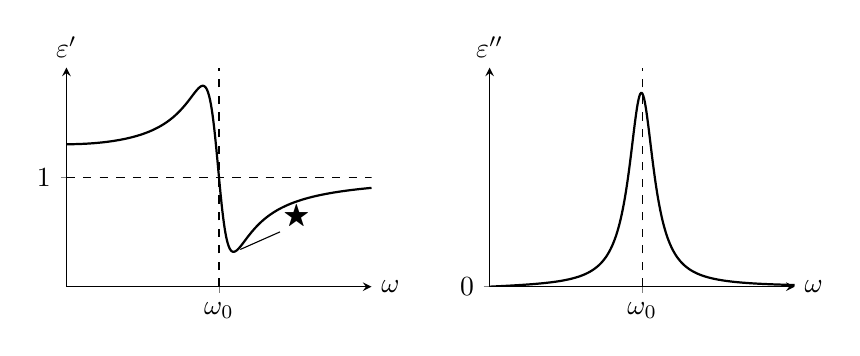
\begin{tikzpicture}
		\begin{axis}[
			name=epsr, width=0.45\textwidth, height=0.36\textwidth,
			axis lines=left, xmin=0, xmax=2, ymin=0, ymax=2,
			xtick={1}, xticklabels={$\omega_0$}, ytick={1},
			xlabel={$\omega$}, ylabel={$\varepsilon'$},
			ylabel style={rotate=-90},
			every axis x label/.style={at={(current axis.right of origin)},anchor=west},
			every axis y label/.style={at={(current axis.above origin)},anchor=south},
			]
			\addplot[dashed, thin, domain=0:2] {1};
			\addplot[dashed, thin] coordinates {(1,0) (1,2)};
			\addplot[thick, samples=400, domain=0:2] {1 + 0.3*(1 - x^2)/((x^2 - 1)^2 + (0.2*x)^2)};
			\draw[thin] (axis cs:1.14,0.34) -- (axis cs:1.4,0.5) node[anchor=south west, inner sep=1pt] {$\bigstar$};
		\end{axis}
		\begin{axis}[
			at={(epsr.east)}, anchor=west, xshift=1.5cm,
			width=0.45\textwidth, height=0.36\textwidth,
			axis lines=left, xmin=0, xmax=2, ymin=0, ymax=1.7,
			xtick={1}, xticklabels={$\omega_0$}, ytick={0},
			xlabel={$\omega$}, ylabel={$\varepsilon''$},
			every axis x label/.style={at={(current axis.right of origin)},anchor=west},
			every axis y label/.style={at={(current axis.above origin)},anchor=south},
			]
			\addplot[dashed, thin] coordinates {(1,0) (1,1.7)};
			\addplot[thick, samples=400, domain=0:2] {0.3*0.2*x/((x^2 - 1)^2 + (0.2*x)^2)};
		\end{axis}
	\end{tikzpicture}
	\caption{Permittivity $\varepsilon'$ (left) and loss factor $\varepsilon''$ (right) of the damped harmonic oscillator model, Eq.~\eqref{e:oscillator}.}
	\label{f:oscillator}
\end{figure}

$\bigstar$ Note that $\varepsilon' < 1$ just above the resonance frequency, even though we mentioned before that $\varepsilon' \ge 1$. Is this a problem? Not really. First, our model is highly simplified, and other mechanisms can act to increase $\varepsilon'$ in real materials. Second, we'll cover this later, but suffice to say for now that energy travels at a maximum speed, and the above does not interfere with that.

%%%%%%%%%%%%%%%%%%%%%%%%%%%%%%%%%%%%%
\section{Properties of natural materials}

\begin{itemize}
	\item The preceding discussion is a simplified model meant to build intuition. Like any classical approach to quantum phenomena, it is an approximation, but it turns out to be a really good one. More rigorous approaches using quantum mechanics yield similar results for the form of $\varepsilon(\omega)$.
	\item It's also worth pointing out that you can take essentially the same approach and then apply Ohm's law to get an expression for the conductivity $\sigma(\omega)$.
	\item Dependence on physical properties like temperature $T$ is implicit in the previous model. This will come into the damping coefficient $\nu$ and the natural frequency $\omega_0$.
\end{itemize}

\subsection{Temperature dependence}

\begin{itemize}
	\item \emph{Permittivity.} We discussed before how atomic vibrations (heat) influence the polarizability (alignment of charges along the electric field) of materials. Permittivity is a description of polarizability, and thus will be a function of $T$.
	% NOTE: handwritten reads "T-dependence of conductivity varies depending on the material, primarily whether heat is conducted by
	% carrier charges or through mechanistic processes (e.g., phonons)"; rewritten in terms of carrier number and scattering, with
	% the metals/semiconductors/electrolytes sentences and the name Wiedemann--Franz added.
	\item \emph{Conductivity.} The $T$-dependence of conductivity varies depending on the material, primarily through how the number of free charge carriers (electrons or ions) and the rate at which they scatter change with temperature. In metals, the number of free electrons is essentially fixed, and stronger lattice vibrations (phonons) at higher $T$ scatter them more often, so $\sigma$ decreases with increasing $T$. In semiconductors and electrolytic solutions like seawater, higher $T$ frees more carriers or makes ions more mobile, so $\sigma$ increases with $T$. We won't get into details in this course, but suffice to say that conductivity will have some $T$-dependence. The classic example is for metals, where electrical and thermal conductivity are linked by the Wiedemann--Franz law (cf.\ Drude theory)
	\begin{equation}
		\sigma = \frac{K}{LT},
	\end{equation}
	where
	\begin{itemize}
		\item $K$ is the thermal conductivity,
		\item $L = \frac{3}{2}\left(\frac{k_B}{e}\right)^2 \approx 1.11\times10^{-8}$ W$\,\Omega$/K$^2$ is the Lorenz number from classical Drude theory (note: the quantum-mechanical (Sommerfeld) treatment gives $L = \frac{\pi^2}{3}\left(\frac{k_B}{e}\right)^2 \approx 2.44\times10^{-8}$ W$\,\Omega$/K$^2$, which agrees better with measurements for most metals),
		\item $k_B$ is the Boltzmann constant, and
		\item $e$ is the electron charge.
	\end{itemize}
	This relation \emph{only} holds for metals but, again, we should expect that conductivity depends on $T$ for all materials.
\end{itemize}

%%%%%%%%%%%%%%%%%%%%%%%%%%%%%%%%%%%%%
\section{Practical example: H$_2$O as pure liquid, liquid with salt, and solid}
\label{s:water}

% NOTE: the generic relaxation time is written tau_rel (handwritten: tau) so that bare tau is free for the Fresnel
% transmission coefficient (Lecture 4; master table D18). Specific relaxation times keep their subscripts (tau_w, tau_i).
In RS applications, it is common to focus on specific frequency ranges corresponding to the instrument, and to consider dielectric properties in terms of a characteristic relaxation time $\tau_\mathrm{rel}$ corresponding to a specific polarization mechanism.
% NOTE: handwritten has tau ~ 1/gamma (damping coefficient, renamed nu here). In the overdamped limit (nu >> omega, omega_0) the oscillator model reduces to
% eps = 1 + (omega_p^2/omega_0^2)/(1 + j omega nu/omega_0^2), i.e., Debye form with tau = nu/omega_0^2.
% NOTE (instructor decision, 2026-09-29): both limits stated. Free carriers (omega_0 = 0): sigma(omega) = eps_0 omega_p^2/(nu + j omega),
% so tau_rel = 1/nu (the handwritten tau ~ 1/gamma). Bound charges, heavily damped: tau_rel = nu/omega_0^2.
The relaxation time depends on the damping $\nu$ of the oscillator model above. For free charges (no restoring force, $\omega_0 = 0$), $\tau_\mathrm{rel} = 1/\nu$, the mean time between collisions. For bound charges in the heavily damped limit ($\nu \gg \omega_0, \omega$), the oscillator model takes the Debye form below with $\tau_\mathrm{rel} \approx \nu/\omega_0^2$.

\subsection{Pure (distilled) water at microwave frequencies ($\omega/2\pi \le 50$ GHz)}

\begin{itemize}
	\item The most common model used in RS (at microwave frequencies) is the \emph{Debye model} (named for Peter Debye). This takes a form very similar to the model we derived for harmonic oscillators:
	\begin{equation}
		\varepsilon = \varepsilon_{w\infty} + \frac{\varepsilon_{w0} - \varepsilon_{w\infty}}{1 + j\omega\tau_w} = \varepsilon' - j\varepsilon'',
	\end{equation}
	where
	\begin{itemize}
		\item $\varepsilon_{w\infty} = \varepsilon(\omega\to\infty)$ is the high-frequency limit,
		\item $\varepsilon_{w0} = \varepsilon(\omega = 0)$ is the nominal or low-frequency limit (note that $\varepsilon_{w0} \ne \varepsilon_0$), and
		\item $\tau_w$ is the relaxation time.
	\end{itemize}
	\item We can break this into real and imaginary components (note the similarity with the harmonic model):
	\begin{equation}
		\varepsilon' = \varepsilon_{w\infty} + \frac{\varepsilon_{w0} - \varepsilon_{w\infty}}{1 + (\omega\tau_w)^2},
		\qquad
		\varepsilon'' = \frac{\omega\tau_w(\varepsilon_{w0} - \varepsilon_{w\infty})}{1 + (\omega\tau_w)^2}.
	\end{equation}
	\item $T$-dependence comes into the model through $\varepsilon_{w0}$ and $\tau_w$, which are invariant over the given range of frequencies ($\omega/2\pi \le 50$ GHz).
	\begin{itemize}
		\item $\varepsilon_{w0}(T)$ and $\tau_w(T)$ are empirical, commonly given as third-order polynomials in $T$. More on this in problem set 1.
		\item $\varepsilon_{w\infty}$ is weakly dependent on $T$; experiments show $\varepsilon_{w\infty} \approx 4.9$ for all $T$.
	\end{itemize}
	\item See the plot and further notes on slide 4 of the lecture slides.
\end{itemize}

\subsection{Salt water}

\begin{itemize}
	\item To account for the effects of ionizing salt on the dielectric constant of water, it is common to use a so-called \emph{double-Debye} dielectric model.
	\item This model takes into account multiple polarizing mechanisms and the conductivity allowed by the presence of salt:
	% NOTE: handwritten has (eps_w0 - eps_winf) in the numerators of the second relaxation terms and (omega tau_w2) unsquared
	% in the second denominator of eps''. Corrected to (eps_w1 - eps_winf) and (omega tau_w2)^2 so that eps'(omega=0) = eps_w0.
	% Ulaby & Long (2014) Eq. (4.19a,b) also print (eps_w0 - eps_winf), but that is a typo in the book: with their Table 4-1
	% coefficients (T = 20 C, S = 0, f = 1 GHz) the printed form gives eps' ~ 154, whereas their Fig. 4-2 shows ~80;
	% the (eps_w1 - eps_winf) form gives 79.9 and reproduces their f02 = 281.4 GHz.
	\begin{align}
		\varepsilon' &= \varepsilon_{w\infty} + \frac{\varepsilon_{w0} - \varepsilon_{w1}}{1 + (\omega\tau_{w1})^2} + \frac{\varepsilon_{w1} - \varepsilon_{w\infty}}{1 + (\omega\tau_{w2})^2}, \\
		\varepsilon'' &= \frac{\omega\tau_{w1}(\varepsilon_{w0} - \varepsilon_{w1})}{1 + (\omega\tau_{w1})^2} + \frac{\omega\tau_{w2}(\varepsilon_{w1} - \varepsilon_{w\infty})}{1 + (\omega\tau_{w2})^2} + \frac{\sigma}{\omega\varepsilon_0},
	\end{align}
	where $\varepsilon_0$ is the permittivity of free space (reminder: $\varepsilon_{w0} \ne \varepsilon_0$).
	\item In this model, $\varepsilon_{w1}$ is $\varepsilon$ at some intermediate frequency (details not important here), and all variables are given as empirical functions of $T$ and salinity $S$.
	% Values computed from Ulaby & Long (2014) Eq. (4.21e) and Table 4-1: eps_winf = a16 + a17*T + a18*S.
	\item Note that $\varepsilon_{w\infty}$ in this model differs from the value $\varepsilon_{w\infty} \approx 4.9$ used in the single-Debye model for pure water. Here, $\varepsilon_{w\infty}$ is an empirical function of $T$ and $S$, ranging from about 3.7 to 4.0 for fresh water ($S = 0$, $0 \le T \le 30^\circ$C) and about 2.8 to 3.1 for typical seawater ($S = 35$ psu). Each value of $\varepsilon_{w\infty}$ belongs to its own model, so the two should not be mixed.
	% NOTE: handwritten cites "Ulaby and Long (2015)"; the existing EM notes cite the same book as 2014.
	\item See Ulaby and Long (2014), Chapter 4, for details.
	\item The take-away from this model is the simple summation of the effects of multiple mechanisms and the explicit treatment of conductivity in the loss factor (see slide 5 of the lecture slides).
	\begin{itemize}
		\item Such models are ubiquitous in RS, so many of you will see these things again in your research.
	\end{itemize}
\end{itemize}

\subsection{Freshwater ice}

\begin{itemize}
	\item Let's recall that we can classify the mechanisms that govern permittivity mainly as rotating or stretching.
	\begin{itemize}
		\item In our capacitor example from before, we illustrated rotation of dipoles, and we just discussed practical, empirical models that consider the characteristic time it takes for dipoles to rotate (relaxation time).
		\item It's easy to imagine how dipoles in gas and liquid states can rotate.
		\item But solids are distinguished from liquids and gases by having an orderly structure.
		\item Water ice has a simple crystalline structure that gives rise to fascinating mechanical properties.
		\begin{itemize}
			\item Due to hydrogen bonding, ice (under terrestrial conditions) forms hexagonal crystals.
			% NOTE: handwritten reads "prevent rotation"; softened because ice does relax, slowly (kHz relaxation frequency, U&L p. 127).
			\item The bonds that form hexagonal crystals strongly hinder rotation of H$_2$O molecules in response to an applied electric field, so the molecules can reorient only very slowly.
		\end{itemize}
	\end{itemize}
	% NOTE: handwritten reads "Models of permittivity in ice, therefore, essentially omit dipole rotation mechanisms"; the reason
	% (slow rotation) was added.
	\item Because dipole rotation in ice is so slow, it contributes little at the frequencies used in most RS applications, and models of permittivity in ice often neglect it. For microwave RS applications (the most common for studying ice properties), this effectively means that
	\begin{equation}
		\varepsilon' \approx 3.2 \quad \text{(virtually independent of $T$ and $\omega$)},
		\qquad
		% NOTE: handwritten has "=" here; Ulaby & Long (2014) Eq. (4.22b) give this as the omega*tau_i >> 1 approximation.
		\varepsilon'' \approx \frac{\varepsilon_{i0} - \varepsilon_{i\infty}}{\omega\tau_i},
	\end{equation}
	where the variables follow the same basic definitions as for pure water.
	% NOTE: the following two sentences are added. The first explains the approximation; the second adds the infrared term
	% (U&L Eq. 4.24, p. 128), which the handwriting omits. At -10 C and 10 GHz the infrared term is ~7.5e-4 vs ~2.7e-5
	% for the Debye tail (U&L Eqs. 4.25a-c).
	The approximation for $\varepsilon''$ holds because $\omega\tau_i \gg 1$ at microwave frequencies; the slow rotation of H$_2$O molecules in ice puts its relaxation frequency in the kilohertz range, so microwave RS sees only the high-frequency tail of this mechanism. This Debye tail dominates $\varepsilon''$ only below about 1--3 GHz. At higher frequencies, an infrared absorption term that increases in proportion to frequency takes over, so that $\varepsilon''$ of ice has a minimum near 1 GHz and rises with frequency above it (Ulaby and Long, 2014, Eq.~4.24 and Fig.~4-3).
	\item Impurities can be added to this model. See slide 6 in this lecture for more details.
\end{itemize}

%%%%%%%%%%%%%%%%%%%%%%%%%%%%%%%%%%%%%
\section{Summary}

\begin{itemize}
	\item We just covered a \emph{ton} of material.
	\item For some of you, this is review with a few new pieces thrown in.
	\item For some of you, this is almost all new. If you felt lost, ask questions.
	\item Overview of key take-aways:
	\begin{itemize}
		\item In RS, we are most interested in the permittivity and conductivity of materials.
		\item Conductivity is a measure of a material's ability to allow electric current (flow of charges: electrons or ions).
		\item Permittivity is, for all intents and purposes, a measure of capacitance, i.e., the polarizability of the atoms and molecules that make up the substance.
		\item There are multiple polarization mechanisms, most of which involve rotating or stretching and are dominant at different EM frequencies:
		\begin{itemize}
			\item \emph{stretching}
			\begin{itemize}
				\item highest $\omega$ $\rightarrow$ electronic (or atomic) polarization
				\item high $\omega$ $\rightarrow$ ionic polarization
			\end{itemize}
			\item \emph{rotation}
			\begin{itemize}
				\item low $\omega$ $\rightarrow$ dipole rotation
			\end{itemize}
			\item \emph{charge accumulation}
			\begin{itemize}
				\item lowest $\omega$ $\rightarrow$ interfacial polarization (charge build-up at boundaries)
			\end{itemize}
		\end{itemize}
	\end{itemize}
\end{itemize}

%%%%%%%%%%%%%%%%%%%%%%%%%%%%%%%%%%%%%
% Symbols follow the master table in ../variables_master.tex; see it for flagged dual usages.
\section*{Variables}

Units are SI. Values are given for universal constants; ``typical'' values are representative, not definitive.

{\small
\renewcommand{\arraystretch}{1.25}
\begin{longtable}{>{$}l<{$} >{\raggedright\arraybackslash}p{0.38\textwidth} >{\raggedright\arraybackslash}p{0.15\textwidth} >{\raggedright\arraybackslash}p{0.24\textwidth}}
\hline
\textrm{Symbol} & Description & Units & Value \\
\hline
\endfirsthead
\hline
\textrm{Symbol} & Description & Units & Value \\
\hline
\endhead
\hline
\endfoot
\multicolumn{4}{l}{\emph{Universal constants}} \\
\varepsilon_0 & permittivity of free space & F/m & $8.854\times10^{-12}$ \\
\mu_0 & permeability of free space & H/m & $4\pi\times10^{-7} \approx 1.257\times10^{-6}$ \\
c & speed of light in a vacuum, $1/\sqrt{\mu_0\varepsilon_0}$ & m/s & $2.998\times10^{8}$ \\
e & elementary (electron) charge (magnitude) & C & $1.602\times10^{-19}$ \\
k_B & Boltzmann constant & J/K & $1.381\times10^{-23}$ \\
j & imaginary unit, $j^2 = -1$ (time dependence $e^{j\omega t}$) & -- & -- \\
\multicolumn{4}{l}{\emph{Constitutive parameters and dielectric properties}} \\
\varepsilon & complex dielectric constant (relative), $\varepsilon' - j\varepsilon''$ & dimensionless & -- \\
\varepsilon' & relative permittivity (real part of $\varepsilon$) & dimensionless & $\ge 1$ (almost always); ice $\approx 3.2$ \\
\varepsilon'' & dielectric loss factor (negative imaginary part of $\varepsilon$) & dimensionless & $\sigma/(\omega\varepsilon_0)$ from conduction \\
\varepsilon_\mathrm{material} & absolute permittivity of a material, $\varepsilon'\varepsilon_0$ & F/m & -- \\
\mu & magnetic permeability & H/m & $\approx\mu_0$ in RS \\
q_v & volume charge density & C/m$^3$ & $0$ in RS \\
\sigma & electrical conductivity & S/m & seawater: $\approx 4.8$ (20$^\circ$C, 35 psu) \\
\omega & angular frequency of the EM wave & rad/s & -- \\
f & frequency, $\omega/2\pi$ & Hz & -- \\
\multicolumn{4}{l}{\emph{Parallel-plate capacitor}} \\
A & plate area & m$^2$ & -- \\
h & plate separation & m & -- \\
Q & charge on each plate & C & -- \\
E & electric field magnitude & V/m & -- \\
\tilde{E} & phasor (complex amplitude) of an oscillating field, $E(t) = \mathrm{Re}[\tilde{E}e^{j\omega t}]$ & V/m & -- \\
E_+,\ E_- & fields produced by the positive and negative plates & V/m & $Q/(2A\varepsilon_0)$ each \\
E_{\mathrm{H_2O}} & field of an aligned water dipole & V/m & -- \\
V & potential difference between the plates & V & -- \\
C & capacitance & F & -- \\
\multicolumn{4}{l}{\emph{Damped harmonic oscillator model}} \\
\xi & particle displacement & m & -- \\
\tilde{\xi} & complex amplitude of $\xi$, $\xi(t) = \mathrm{Re}[\tilde{\xi}e^{j\omega t}]$ & m & -- \\
m & mass of the bound particle & kg & -- \\
q & charge of the bound particle & C & -- \\
K_\mathrm{spring} & effective spring constant of the bond & N/m & $m\omega_0^2$ \\
\omega_0 & natural (resonant) angular frequency & rad/s & -- \\
\nu & damping coefficient & s$^{-1}$ & -- \\
F_\mathrm{bond} & restoring (bond) force & N & -- \\
F_\mathrm{damping} & damping force & N & -- \\
F_\mathrm{driving} & driving force from the oscillating field & N & -- \\
p,\ \tilde{p} & dipole moment, $q\xi$, and its phasor, $q\tilde{\xi}$ & C$\cdot$m & -- \\
P,\ \tilde{P} & polarization (dipole moment per unit volume), $Np$, and its phasor & C/m$^2$ & -- \\
N & number of dipoles per unit volume & m$^{-3}$ & -- \\
\omega_p & plasma frequency, $\omega_p^2 = Nq^2/(\varepsilon_0 m)$ & rad/s & -- \\
\tau_\mathrm{rel} & characteristic relaxation time of a polarization mechanism & s & $1/\nu$ (free charges); $\approx\nu/\omega_0^2$ (bound, overdamped) \\
\multicolumn{4}{l}{\emph{Temperature dependence}} \\
T & temperature & K ($^\circ$C in empirical fits) & -- \\
K & thermal conductivity & W\,m$^{-1}$\,K$^{-1}$ & -- \\
L & Lorenz number & W\,$\Omega$\,K$^{-2}$ & Drude: $1.11\times10^{-8}$; Sommerfeld: $2.44\times10^{-8}$ \\
\multicolumn{4}{l}{\emph{Water and ice}} \\
\varepsilon_{w0} & static (low-frequency) dielectric constant of water & dimensionless & 88.0 (0$^\circ$C), 80.1 (20$^\circ$C) \\
\varepsilon_{w\infty} & high-frequency dielectric constant of water & dimensionless & 4.9 (single-Debye); 2.8--4.0 (double-Debye) \\
\varepsilon_{w1} & intermediate-frequency dielectric constant (double-Debye) & dimensionless & -- \\
\tau_w & relaxation time of pure water & s & $1.8\times10^{-11}$ (0$^\circ$C), $9.3\times10^{-12}$ (20$^\circ$C) \\
\tau_{w1},\ \tau_{w2} & relaxation times of the two double-Debye terms & s & -- \\
S & salinity & psu (\textperthousand) & seawater $\approx 35$ \\
\varepsilon_{i0},\ \varepsilon_{i\infty} & static and high-frequency dielectric constants of ice & dimensionless & -- \\
\tau_i & relaxation time of ice & s & relaxation frequency in kHz range \\
\end{longtable}
}

\end{document}
